\documentclass{beamer}
\setbeamertemplate{footline}[page number]
\date{}
\author{}
\institute{}

%%%%%%% Put these names back in the final version 
%\\Aswathy Rajendra Kurup\\Meenu Ajith}
%\institute{Department of Electrical and Computer Engineering\\The University of New Mexico}
\setbeamercovered{transparent}
\usepackage{setspace}
\usepackage{array}
\usepackage[T1]{fontenc}
\usepackage{graphicx}
\usepackage{amsmath}
\usepackage{amsfonts}
\usepackage{amssymb}
\usepackage{makeidx}
\usefonttheme{serif}
\usepackage{multirow}
\usepackage{booktabs} 
\usepackage{rotating}
\usepackage{color}
\usepackage{float}
\usepackage[latin1]{inputenc}
\usepackage[english]{babel}
\usepackage{amsmath}
\usepackage{amsfonts}
\usepackage{eurosym}
\usepackage{rotating}
\usepackage{multicol}
\usepackage{pythonhighlight}
\usepackage[normalem]{ulem}
\newcommand{\ba}{{\bf a}}
\newcommand{\bb}{{\bf b}}
\newcommand{\bc}{{\bf c}}
\newcommand{\bd}{{\bf d}}
\newcommand{\be}{{\bf e}}
\newcommand{\bbf}{{\bf f}}
\newcommand{\bg}{{\bf g}}
\newcommand{\bh}{{\bf h}}
\newcommand{\bi}{{\bf i}}
\newcommand{\bk}{{\bf k}}
\newcommand{\bl}{{\bf l}}
\newcommand{\bm}{{\bf m}}
\newcommand{\bn}{{\bf n}}
\newcommand{\bo}{{\bf o}}
\newcommand{\bp}{{\bf p}}
\newcommand{\bq}{{\bf q}}
\newcommand{\br}{{\bf r}}
\newcommand{\bs}{{\bf s}}
\newcommand{\bt}{{\bf t}}
\newcommand{\bu}{{\bf u}}
\newcommand{\bv}{{\bf v}}
\newcommand{\bw}{{\bf w}}
\newcommand{\bx}{{\bf x}}
\newcommand{\by}{{\bf y}}
\newcommand{\bz}{{\bf z}}

\newcommand{\bA}{{\bf A}}
\newcommand{\bB}{{\bf B}}
\newcommand{\bC}{{\bf C}}
\newcommand{\bE}{{\bf E}}
\newcommand{\bG}{{\bf G}}
\newcommand{\bH}{{\bf H}}
\newcommand{\bI}{{\bf I}}
\newcommand{\bK}{{\bf K}}
\newcommand{\bL}{{\bf L}}
\newcommand{\bM}{{\bf M}}
\newcommand{\bO}{{\bf O}}
\newcommand{\bQ}{{\bf Q}}
\newcommand{\bR}{{\bf R}}
\newcommand{\bS}{{\bf S}}
\newcommand{\bT}{{\bf T}}
\newcommand{\bV}{{\bf V}}
\newcommand{\bW}{{\bf W}}
\newcommand{\bX}{{\bf X}}
\newcommand{\bY}{{\bf Y}}
\newcommand{\bZ}{{\bf Z}}
\newcommand\uptocnt{\stackrel{\mathclap{\normalfont\mbox{c}}}{\propto}}
\newcommand{\bpt}{{\bf pt}}
\newcommand{\bpl}{{\bf pl}}
\newcommand{\bdp}{{\bf dp}}
\newcommand{\btemp}{{\bf temp}}

\newcommand{\bmu}{{\boldsymbol \mu}}
\newcommand{\bSigma}{{\boldsymbol \Sigma}}
\newcommand{\bsigma}{{\boldsymbol \sigma}}
\newcommand{\bvarPhi}{{\boldsymbol \varPhi}}
\newcommand{\bvarphi}{{\boldsymbol \varphi}}
\newcommand{\bPhi}{{\boldsymbol \Phi}}
\newcommand{\bdelta}{{\boldsymbol \delta}}
\newcommand{\bZero}{{\bf 0}}
\newcommand{\bOne}{{\bf 1}}
\newcommand{\balpha}{{\boldsymbol \alpha}}
\newcommand{\bAlpha}{{\boldsymbol A}}
\newcommand{\btheta}{{\boldsymbol \theta}}

\newcommand{\softmax}{\text{softmax}}
\newcommand{\diag}{\text{diag}}
\newcommand{\sinc}{\mathrm{sinc}}
\newcommand{\argmin}{\mathop{\mathrm{argmin}}}
\newcommand{\infl}{\eta}
\newcommand{\Ind}{\mathrm{I}}
\newcommand{\Real}{\mathbb R}
\newcommand{\Intg}{\mathbb Z}
\newcommand{\Complex}{\mathbb C}
\newcommand{\Natural}{\mathbb N}
\newcommand{\Fourier}[1]{\mathcal{F} \{#1\}}
%\newcommand{\ii}{\mathbbm{i}}
\newcommand{\bphi}{\boldsymbol{\mathit{\phi}}}

\newcommand{\hs}{\hspace{2pt}}
\newcommand{\sign}{\text{sign}}
\author{Manel Mart\'inez-Ram\'on\\Meenu Ajith\\Aswathy Rajendra Kurup}

\usetheme{Madrid}
\usecolortheme{beaver}
\usepackage{tikz}
\usetikzlibrary{fit,arrows,calc,positioning}
\usepackage{listings}
\usepackage{xcolor}
\usepackage{emerald} 
\usepackage[T1]{fontenc} 
\usepackage{verbatim}
\usepackage{graphicx}
\usepackage{epsfig}
\usepackage{psfrag}
\usepackage[english]{babel}
\usepackage{listings}
\usepackage{courier}
\usepackage{color}
 \usepackage{vwcol} 
 \usepackage[english]{babel} % To obtain English text with the blindtext package
\usepackage{blindtext}
\definecolor{codegreen}{rgb}{0,0.6,0}
\definecolor{codegray}{rgb}{0.5,0.5,0.5}
\definecolor{codepurple}{rgb}{0.58,0,0.82}
\definecolor{backcolour}{rgb}{0.95,0.95,0.92}

\lstdefinestyle{mystyle}{
  backgroundcolor=\color{backcolour},   commentstyle=\color{codegreen},
  keywordstyle=\color{magenta},
  numberstyle=\tiny\color{codegray},
  stringstyle=\color{codepurple},
  basicstyle=\ttfamily\footnotesize,
  breakatwhitespace=false,         
  breaklines=true,                 
  captionpos=b,                    
  keepspaces=true,                 
  numbers=left,                    
  numbersep=5pt,                  
  showspaces=false,                
  showstringspaces=false,
  showtabs=false,                  
  tabsize=2
}
\lstset{style=mystyle}

%% Stuff for movies

% %\newcommand{\bt}{{\bf t}}
% \newcommand{\br}{{\bf r}}
% \newcommand{\bs}{{\bf s}}
% \newcommand{\by}{{\bf y}}
% \newcommand{\bz}{{\bf z}}
% \newcommand{\bx}{{\bf x}}
% \newcommand{\bw}{{\bf w}}
% \newcommand{\be}{{\bf e}}
% \newcommand{\bbf}{{\bf f}}
% \newcommand{\bb}{{\bf b}}
% \newcommand{\bd}{{\bf d}}
% \newcommand{\bA}{{\bf A}}
% \newcommand{\bB}{{\bf B}}
% \newcommand{\bL}{{\bf L}}
% \newcommand{\bM}{{\bf M}}

% \newcommand{\bC}{{\bf C}}
% \newcommand{\bI}{{\bf I}}
% \newcommand{\bK}{{\bf K}}
% \newcommand{\bk}{{\bf k}}
% \newcommand{\bT}{{\bf T}}
% \newcommand{\bV}{{\bf V}}
% \newcommand{\bW}{{\bf W}}
% \newcommand{\bX}{{\bf X}}
% \newcommand{\bY}{{\bf Y}}
% \newcommand{\bZ}{{\bf Z}}
% \newcommand{\bm}{{\bf m}}
% \newcommand{\bpt}{{\bf pt}}
% \newcommand{\bpl}{{\bf pl}}
% \newcommand{\bdp}{{\bf dp}}
% \newcommand{\btemp}{{\bf temp}}
% \newcommand{\bl}{{\bf l}}
% \newcommand{\bu}{{\bf u}}
% \newcommand{\bmu}{{\boldsymbol \mu}}
% \newcommand{\bSigma}{{\boldsymbol \Sigma}}
% \newcommand{\bLambda}{{\boldsymbol \Lambda}}

% \newcommand{\bsigma}{{\boldsymbol \sigma}}
% \newcommand{\bvarphi}{{\boldsymbol \varPhi}}
% \newcommand{\btheta}{{\boldsymbol \theta}}
% \newcommand{\bZero}{{\bf 0}}
% \newcommand{\balpha}{{\boldsymbol \alpha}}
% \newcommand{\bpi}{{\boldsymbol \pi}}
% \newcommand{\bxi}{{\boldsymbol \xi}}
% \newcommand{\bdelta}{{\boldsymbol \delta}}
\lstset{
	language=Python,
	basicstyle=\footnotesize\ttfamily\color{black},
	commentstyle = \footnotesize\ttfamily\color{red},
	keywordstyle=\footnotesize\ttfamily\color{blue},
	stringstyle=\footnotesize\ttfamily\color{black},
%	columns=fixed,
%	numbers=left,    
	numberstyle=\tiny,
	stepnumber=1,
	numbersep=5pt,
	tabsize=1,
	extendedchars=true,
	breaklines=true,            
	frame=b,         
	showspaces=false,
	showtabs=true,
	xleftmargin=6pt,
	framexleftmargin=6pt,
	framexrightmargin=2pt,
	framexbottommargin=4pt,
	showstringspaces=false      
}

\lstloadlanguages{
         Python
}

%\graphicspath{ {./images/} }  % Figures path - used in graphicx

%\selectcolormodel{cmyk}

\mode<presentation>

\newcommand{\dred}{darkred!90!black}
\newcommand{\written}{\ECFJD\textcolor{cyan!50!white}}
\newcommand{\hlight}{\textcolor{\dred}}
\newcommand{\Ex}{\textcolor{\dred}{Ex. }}

% remove navigation symbols in full screen mode
\setbeamertemplate{navigation symbols}{}  
\setbeamertemplate{blocks}[rounded][shadow=false]
\setbeamercolor{note page}{fg=black}

\setbeamercolor{title}{fg=\dred}
\setbeamercolor{frametitle}{fg=white}
\setbeamercolor{frametitle}{bg=\dred}
\setbeamercolor{structure}{fg=black,bg=white}
\setbeamercolor{background canvas}{bg=white,fg=black}
\setbeamercolor{normal text}{fg=black,bg=white}
\setbeamercolor{item}{fg=red!80!black,bg=white!}
\addtobeamertemplate{block begin}{\setbeamercolor{block title}{fg=white,bg=\dred}
\setbeamercolor{block body}{fg=white,bg=gray}}{}


\usepackage{algorithm,algorithmic}
\usepackage[algo2e]{algorithm2e} 
%\title{Lesson 1.1}
\title{1. Feedforward neural networks}
\subtitle{1.3a. The Backpropagation algorithm (1)}


\addtobeamertemplate{frametitle}{}



\begin{document}

\maketitle

\begin{frame}{Introduction}
    \begin{itemize}
        \item So far we have seen the details of the structure of a NN, and its training criterion (maximum likelihood). 
        \item The Backpropagation algorithm implements the criterion over the structure. 
        \item The algorithm is based on a gradient descent strategy. We need to learn:
        \begin{itemize}
            \item The basic algorithm 
            \item Its practical coding
            \item The additions needed to actually make it work.
        \end{itemize}
    \end{itemize}
\end{frame}

\begin{frame}{Gradient descent strategy}
\begin{itemize}
    \item The criterion consists of maximizing the cross entropy between a measured distribution $q(y|\bx)$ of the data and a model  $p(y|\bx)$, implemented as 
    \begin{equation}
    \begin{split}
        J_{ML}(\bY,\bX,\btheta) & = -\mathbb{E} \left[ q\left(\by|\bx\right)\log p\left(\by|\bx \right)\right]\\
        & \approx - \sum_{j} \log p\left(\by_j|\bx_j \right)
    \end{split}
    \end{equation}
\item 
We assume that $q(\cdot)$ is binary, thus the criterion is equivalent to maximize the output likelihood with respect to the data. 
\end{itemize}
\end{frame}

\begin{frame}{Gradient descent strategy}
\begin{itemize}
    \item The goal of the neural network training is to find the maximum of the cross entropy (or the minimum of the negative cross entropy).
    
    \item  The minimum can be found by nulling the gradient of the cost function, The goal is:
    
    \begin{equation}
\frac{\partial J_{ML}({\boldsymbol\theta})}{\partial w^{(l)}_{j,k}} = 0, \forall j,k,l
\end{equation}
    \item This is an equation that cannot be solved in a single step.
    \item We need to proceed in sequential approximations: gradient descent. 
\end{itemize}     
\end{frame}

\begin{frame}{Gradient descent strategy}
\begin{multicols}{2}
    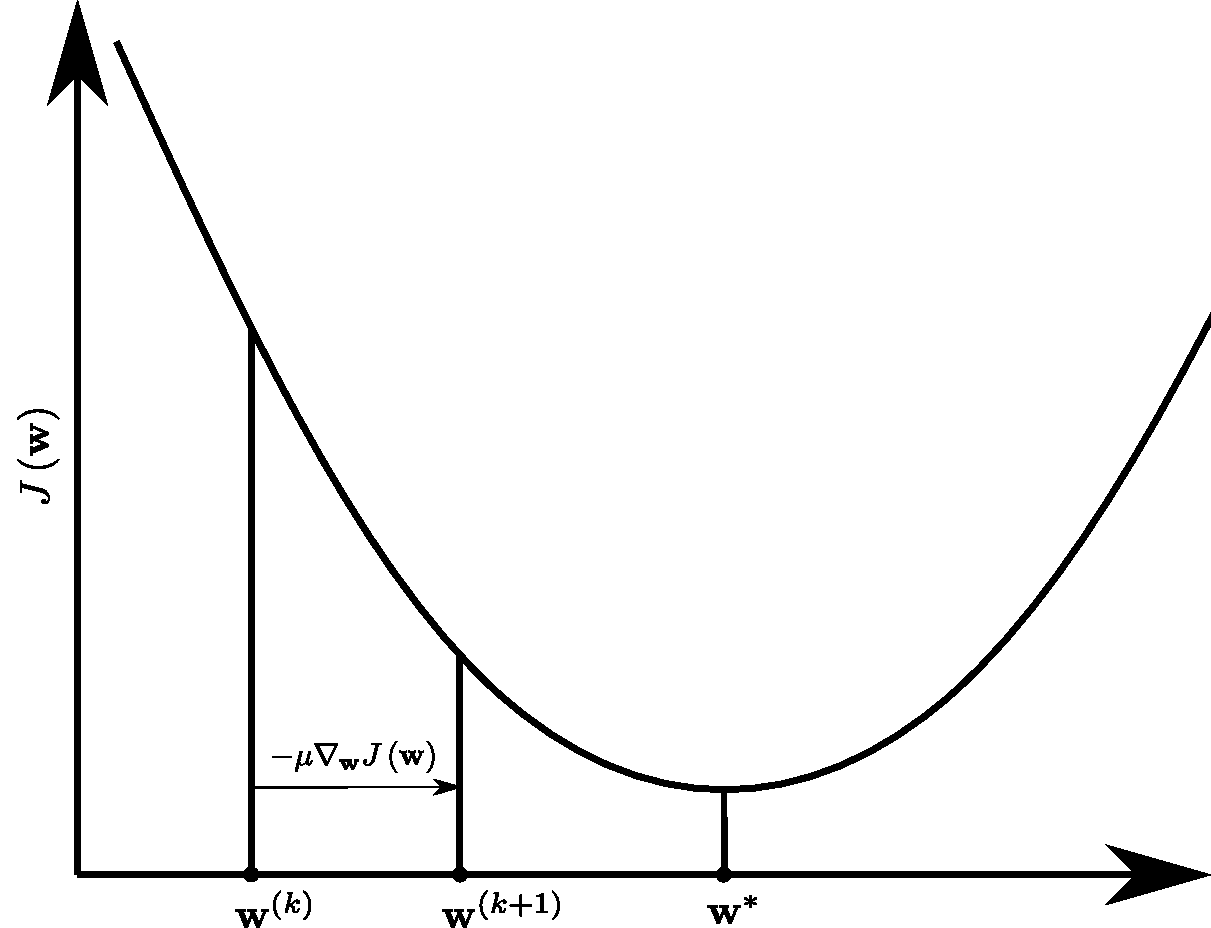
\includegraphics[scale=0.3]{Module 1 (NN)/pics/gradient_descent2.pdf} 
 
 \columnbreak
\begin{itemize}
\item Optimum value $\bw^*$  achieved at the minimum of 
 the cost function, where
$$
\nabla_{\bf w} J_{ML}\left( \bw \right) = 0
$$

\item $\bw^k$ is modified in the direction of the gradient descent times a small constant $\mu$. 

\item The operation must be repeated until the gradient is zero. 
\end{itemize}    
\end{multicols}
\end{frame}

\begin{frame}{Gradient wrt output weigths}

\begin{itemize}
\item Function implemented by the NN as a composition of functions 
\begin{equation}
\begin{split}
    \bbf(\bx)  &=  \bo\left(\bz^{(L)}\right) = \bo\left({\bW^{(L)}}^\top\bh^{(L-1)}\right) \\
    &=\bo\left({\bW^{(L)}}^\top\bphi\left({\bW^{(L-1)}}^\top\bh^{(L-2)}\right)\right)=\cdots
    \end{split}
\end{equation}
\item Derivative wrt the output weights
\begin{equation}
\begin{split}
&\frac{d}{dw_{i,j}^{(L)}}   J_{ML}(\by,\bbf(\bx))= \frac{d}{dw_{i,j}^{(L)}}  J_{ML}\left(\by,\bo\left(\bz^{(L)}\right)\right)=\\ 
&\frac{d}{dw_{i,j}^{(L)}}  J_{ML}\left(\by,\bo\left({\bW^{(L)}}^\top\bh^{(L-1)}\right)\right)
\end{split}
\end{equation} 
\item We assume here that the bias vectors are inside $\bW^{(L)}$
    \end{itemize}
\end{frame}

\begin{frame}{Chain rule}{Output weights}
    \begin{itemize}
        \item The output activation $\bo$ has elements $o_j$ 
        \item $\bz^{(L)} = {\bW^{(L)}}^\top\bh^{(L-1)}$ is a function of the previous layer, with components  $h_i^{(L-1)}$. 
        \item We apply the chain rule to these three elements and to weight $w^{(L)}_{i,j}$.  
\begin{equation}
\frac{dJ_{ML}}{dw_{i,j}^{(L)}}=\frac{dJ_{ML}}{do_{j}} \frac{do_j}{dz_{j}^{(L)}}\frac{dz_j^{(L)}}{dw_{i,j}^{(L)}}
\end{equation}

    \end{itemize}
\end{frame}

\begin{frame}{Chain rule}{Output weights}
\begin{itemize}
    \item We have three terms:
    \vspace{0.5cm}
    \begin{enumerate}
        \item $\frac{d}{do_{j}}J_{ML}$ 
        \vspace{0.5cm}
        \item $\frac{d}{dz_{j}^{(L)}} o_j\left( z_j^{(L)}\right)=o'_j$
        \vspace{0.5cm}
        \item $\frac{d}{dw_{i,j}^{(L)}} z_j^{(L)} = h^{(L-1)}_i$
        \vspace{0.5cm}
    \end{enumerate}
    \item Therefore 
    \begin{equation}\label{eq:deivative_layer_L}
\frac{dJ_{ML}}{dw_{i,j}^{(L)}}= \frac{dJ_{ML}}{do_{j}}{o_j'} h_{i}^{(L-1)} = h_i^{(L-1)}\delta^{(L)}_j 
\end{equation}  
\end{itemize}
\end{frame}

\begin{frame}{Chain rule}{Output weights}

\begin{itemize}
    \item We have used the following definition

\begin{equation}\label{eq:error_term_layer_L}
    \delta^{(L)}_j = \frac{dJ_{ML}}{do_{j}}{o_j'} 
\end{equation}
    
    \item This is element $j$ of vector 
\begin{equation}
    \bdelta^{(L)} = \nabla_{\bo}J_{ML}(\by,\bo) \odot \bo'
\end{equation}
which is the elementwise product $\odot$ of two vectors. 
\end{itemize}
\end{frame}

\begin{frame}{Chain rule}{Output weights}

\begin{itemize}
\item Then, derivative 
\begin{equation}\nonumber
\frac{dJ_{ML}}{dw_{i,j}^{(L)}}= h_i^{(L-1)}\delta^{(L)}_j 
\end{equation}  
is element $i,j$ of a matrix that can be written as $\bh^{(L-1)} \bdelta^{(L)\top}$, thus

\begin{equation}\label{eq:output_gradient}
    \nabla_{\bW^{(L)}} J_{ML} =\bh^{(L-1)} \bdelta^{(L)\top}
\end{equation} 

    
\end{itemize}
    
\end{frame}

\begin{frame}{Weight update}{Output weights}
By using  expression \eqref{eq:output_gradient}, the update of the last layer of the NN consists in the following update operation, 
\begin{equation}\label{eq:update_L}
    \bW^{(L)} \leftarrow     \bW^{(L)}  - \mu   {\bh^{(L-1)}}{\boldsymbol \delta}^{(L)\top} 
\end{equation}
where $\mu$ is a small scalar usually called the learning rate.
\end{frame}

\begin{frame}{Weight update}{Output biases}
\begin{itemize}
    \item Now, what happened with the biases? We put them inside $\bW^{(L)}$
    

 \begin{equation}
    \bW^{(L)} = \left( 
        \begin{array}{cccc}
        \bw^{(L)}_1 & \bw^{(L)}_2 & \cdots &\bw^{(L)}_{D_L} \\
        \\
        b^{(L)}_1 & b^{(L)}_2 & \cdots & b^{(L)}_{D_L}
    \end{array}
    \right)
\end{equation}
   
\item so we redefined $\bh^{(L-1)} = \left( h^{(L-1)}_1~h^{(L-1)}_2~\cdots ~h^{(L-1)}_{D_{L-1} }~1\right)^\top$

\item therefore if   
\begin{equation}\nonumber
\frac{dJ_{ML}}{dw_{i,j}^{(L)}}= h_i^{(L-1)}\delta^{(L)}_j 
\end{equation}
then
\begin{equation}\label{eq:derivative_bias_L}
\frac{dJ_{ML}}{db_{j}^{(L)}}= \delta^{(L)}_j 
\end{equation}  
This is, Eq. \eqref{eq:update_L} is valid without loss of generality.
\end{itemize}
\end{frame}
\end{document}



\begin{frame}{Training a neural network}{Forward step}

The forward step consists of computing all the NN activations for all the training samples. 


\begin{algorithm}[H]
\begin{algorithmic}[1]
\REQUIRE ${\bf X}, {\bf y},{\boldsymbol \theta}$

\FOR{$i=1$ \TO $L$ } 
\STATE {
${\bf h}^{0}={\bf x}_i$
\FOR{$j=1$ \TO $L$} 
\STATE {
${\bf h}^{(j)}=\phi({\bf W}^{(j)\top}{\bf h}^{(j-1)}+{\bf b}^{(j)})$
}
\ENDFOR
} 
\ENDFOR
\STATE $\hat{\bf y}\leftarrow {\bf h}^{(L)}$
\RETURN $\hat{\bf y}$
\end{algorithmic}
\caption{Forward step}\label{alg:forward}
\end{algorithm}
\end{frame}

\begin{frame}{Training a neural network}{Backward step}



The backward step optimizes the structure with respect to all parameters $\boldsymbol\theta : \{w^{(j)}_{i,k},b^{(j)}_{i}\}$ by 
\begin{equation}
\frac{\partial J({\boldsymbol\theta})}{\partial w^{(j)}_{i,k}} = 0
\end{equation}
where usually the cost function is a regularized form of the maximum likelihood.
\end{frame}
\begin{frame}{The chain rule}
The function implemented by the NN can be expressed as 
\begin{equation}
    \bbf(\bx)  =  \bo\left(\bz^{(L)}\right) = \bo\left({\bW^{(L)}}^\top\bh^{(L-1)}\right)= \bo\left({\bW^{(L)}}^\top\phi\left(\bW^{(L-1)}\bh^{(L-2)}\right)\right)\cdots
\end{equation}

 We can express each one of the hidden layer outputs as 
\begin{equation}
    \bh^{(l)}=\phi\left(\bz^{(l)}\right)
\end{equation}
where   $z_i^ {(l)}={\bw_i^{(l)}}^\top \bh^{(l-1)}$.

\end{frame}

\begin{frame}{The chain rule}
By using the chain rule of calculus, we have
\begin{equation}
\begin{split}
&\frac{d}{dw_{i,j}^{(L)}}   J_{ML}(\by,\bbf(\bx))=\\ &=\frac{d}{dw_{i,j}^{(L)}}  J_{ML}\left(\by,\bo\left(\bz^{(L)}\right)\right) \frac{d}{dw_{i,j}^{(L)}}  J_{ML}\left(\by,\bo\left({\bW^{(L)}}^\top\bh^{(L-1)}\right)\right)\\ &=\frac{J_{ML}\left(\by,\bo\left(\bz^{(L)}\right)\right)}{do_{j}} \frac{do_j}{dz_{j}^{(L)}}\frac{dz_j}{dw_{i,j}^{(L)}}
%\\&
= \frac{dJ_{ML}}{do_{j}}{o_j}' h_{i}^{(L)} = \delta^{(L)}_j h_i^{(L-1)}
\end{split}
\end{equation}    
This is element $i,j$ of a matrix that can be written as $\bh^{(L-1)} \bdelta^{(L)\top}$.
where 
\begin{equation}
    \bdelta^{(L)} = \nabla_{\bo}J_{ML}(\by,\bo) \odot \bo'
\end{equation}
\end{frame}



\begin{frame}{The backpropagation}

Using the same reasoning as before, let us now compute the gradient, evaluated for a sample pair $(\bx,~\by)$, of the cost function with respect to weight $w^{(L-1)}_{i,j}$, this is,
\begin{equation}
\begin{split}
    \frac{d}{dw_{i,j}^{(L-1)}}   J_{ML}(\by,\bbf(\bx)) &= \sum_{k,n} \frac{\delta J_{ML}}{do_k}\frac{do_k}{dz_k^{(L)}}\frac{dz_k^{(L)}}{dh_{n}^{(L-1)}}\frac{dh_n^{(L-1)}}{dz_j^{L-1}}\frac{dz^{(L-1)}_j}{dw_{i,j}^{(L-1)}}\\
    &=\sum_{k,m,n} \delta_k^{(L)}w_{k,n}^{(L)}\phi'\left(z^{(L-1)}_j\right)h^{L-2}_i=\delta_j^{(L-1)}h^{(L-2)}_i
    \end{split}
\end{equation}
\end{frame}

\begin{frame}{The backpropagation}
The update of the previous layer, in matrix form, is 

\begin{equation}
    \bW^{(L-1)} \leftarrow     \bW^{(L-1)}  - \mu  {\bh^{(L-2)}} {\boldsymbol \delta}^{(L-1)^\top} - \mu \lambda \bW^{(L-1)}
\end{equation}
where 
\begin{equation}
    {\boldsymbol \delta}^{(L-1)} = \phi'(\bz^{(L-1)})\odot\bW^ {(L)}{\boldsymbol \delta}^{(L)}
\end{equation}


\end{frame}

\begin{frame}{The backpropagation}

If we iterate the process, the update of weight matrix $\bW^{l-1}$ is 
\begin{equation}
    - \mu  {\boldsymbol \delta}^{(l-1)} {\bh^{(l-2)}}^\top - \mu \lambda \bW^{(l-1)}
\end{equation}
where  
\begin{equation}
    {\boldsymbol \delta}^{(l-1)} = \phi'(\bz^{(l-1)})\odot\bW^ {(l)}{\boldsymbol \delta}^{(l)}
\end{equation}
Since local gradients ${\boldsymbol \delta}^{l}$ propagate back to the input, the algorithm is called BP.  
\end{frame}

\begin{frame}{The backpropagation}{Pseudocode}
    
    
    \begin{algorithm}[H]
\begin{algorithmic}[1]
\STATE{${\bf g}\leftarrow \nabla_{\hat{\bf y}}J = \nabla_{\hat{\bf y}}L(\hat{\bf y},{\bf y})$}
\FOR{$j=L$ \TO $1$ } 
\IF{j=l}
\STATE {
${\bf g}\leftarrow {\bf g}\odot o'_j({\bf z}^{(j)})$
} 
\ELSE 
\STATE {
${\bf g}\leftarrow {\bf g}\odot \phi'_j({\bf z}^{(j)})$
} 
\ENDIF

\STATE{
$\nabla_{{\bf W}^{(j)}}L={\bf h}^{(j-1)}{\bf g}^\top + \lambda \bW^{(j)}$
}

\STATE{
$\nabla_{\bb^{(j)}}L={\bf g}^\top + \lambda \bb^{(j)}$
}

\STATE{
${\bf g}\leftarrow {\bf W}^{(j)}{\bf g}$
}
\ENDFOR
\end{algorithmic}
\caption{Backward step (computation of the weight updates)}\label{alg:backpropagation}
\end{algorithm}
    
\end{frame}

\end{document}